\documentclass[10pt, a4paper, twocolumn]{article}
\usepackage{graphicx}
\usepackage{float}

\title{Reconciling organizational cost across business units}
\author{Mya Pitzeruse}

\begin{document}
\maketitle

\begin{abstract}
  This paper describes a solution to reconcile cost for shared infrastructure across business units.
  It was designed to be comprehensive and flexible.
  The original target for the solution was a hybrid-cloud infrastructure.
  As a result, it's concepts are generic and support both cloud and non-cloud ecosystems.
  The goal of the solution is to attribute costs appropriately across a spectrum of platforms.
\end{abstract}


\section*{Introduction}
  Workloads run across a variety of platforms.
  Many systems use a combination of these platforms to perform work efficiently.
  Figure \ref{figure:1} demonstrates how you might use platforms like Apache Hadoop, Kubernetes, and other managed services to build a product.

  \begin{figure}[H]
    \centering
    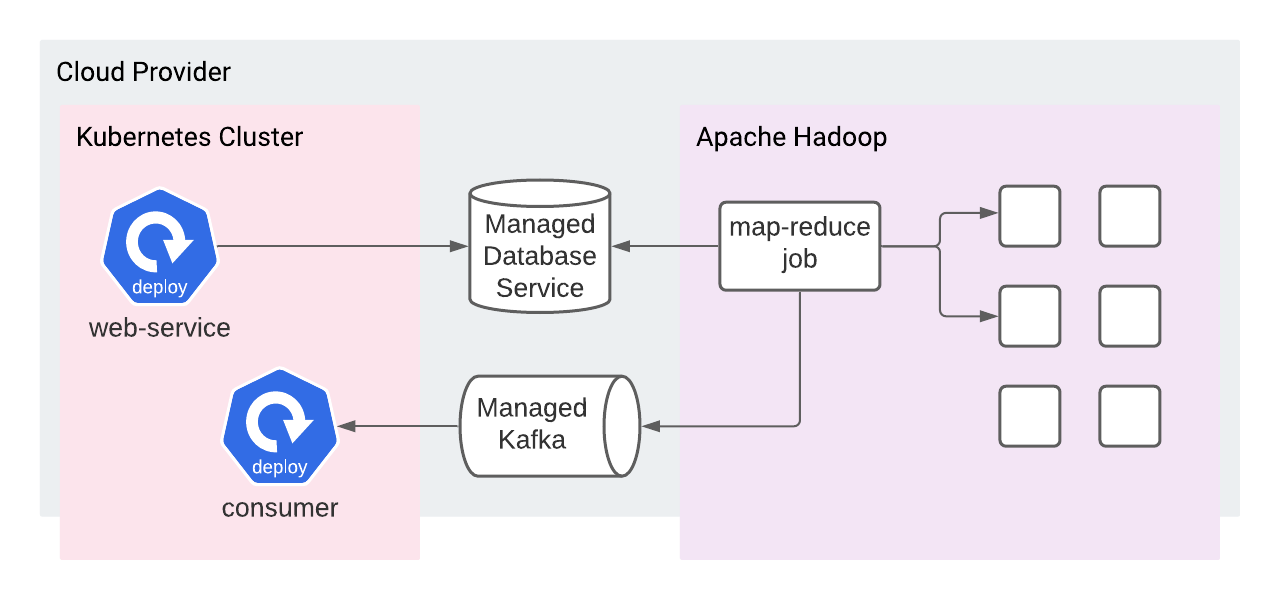
\includegraphics[width=\linewidth]{./truth-and-reconciliation-application.png}
    \caption{A multiple platform application}
    \label{figure:1}
  \end{figure}

  When an organization is small, they're often less concerned about attributing spend to their workloads.
  As an organization grows, they often add new products to complement their existing offerings.
  With each new product, this figure grows more complex.
  As this figure grows more complex, the need to attributing spend increases as well.
  Executives often want to know how much each of their products cost to run and what their return on investment is.
  When asked for this information, engineering leaders need to take time to track down all this information.

  Solutions like CloudTamer help organizations better manage their spend on cloud providers, but lack visibility into clustered environments.
  In cluster solutions like kubecost provide visibility into the cost of Kubernetes workloads, but miss managed resources.
  In the end, you wind up back to where you started.
  Needing to query multiple sources for information.

  While these may represent common cases, it fails to account for less common cases.
  Suppose one part of your organization runs a service on behalf of the rest.
  You might want to apportion usage of that service out to it's heaviest consumers.
  Throughout the course of my research, I found that no (if not few) comprehensive solutions exist.
  In designing a comprehensive solution, I wanted to ensure compatibility with many existing solutions.


\section*{Background}
  In November 2018, I re-joined Indeed to help with their ongoing Kubernetes effort.
  At the time, we were feeling some pain-points scaling our Apache Mesos based infrastructure.
  Some efforts towards a Kubernetes based ecosystem had been underway.

  The first effort was geared toward a short-term migration.
  It would allow us to move off Apache Mesos while preserving the overall structure of our ecosystem.
  The second was tasked with figuring out how to run upstream Kubernetes safely and securely.
  As we underwent these migrations, teams started to build in cost attribution.
  The idea was to use these reports for some comparative analysis when switching platforms.

  Similar questions were raised as we began our journey to the the cloud.
  During this time, I considered several solutions.
  Many of them were geared toward solving in cluster or out of cluster costs, not both.
  In working with the CNCF end user group, I learned many organizations share similar positions.
  Either they were looking for a more comprehensive solution or were using multiple to fill in the gaps.
  At the time, my focus at work was pretty deep into this space.

  In discovering a lack of comprehensive solutions, I researched as much as I could.
  I looked to open source to see what solutions did well and what they were missing.
  I looked at the data we were already reporting and how I could build off that.
  In doing soIn doing so, I was able to identify commonalities across each of them.

  \begin{itemize}
    \item Resources between each data set varied with some commonality (CPU, memory, disk)
    \item Workloads have an identifier, often unique to the platform
    \item Each data set represented an exchange of services between one group and their customers
  \end{itemize}

  These discoveries lead to the design a development of a common reporting platform.
  This platform is designed with decomposition in mind.
  It allows additional layers to be added progressively, allowing organizations to get more granular over time.

\section*{Concepts}
  Much of the solution design is based on these fundamental concepts.

  \subsection*{Resources}
    Workloads require resources to run.
    Common cases need things like CPU, memory, and occasionally disk.
    At the same time, it's important that these resources are made available through a variety of platforms.
    Kubernetes allows containers to reserve resources and it finds room within the cluster to run.
    Similarly, virtual machines can be used to allocate these resources, while also providing virtualized hardware.
    Regardless of where and how the workloads run, resources are uniform.
    They are measured using standardized units and typically come at some cost.

  \subsection*{Standard Units of Measure}
    With anything we measure, standardization and documentation of units is important.
    Without it, one group of engineers might code against one while the others code against another.
    While this paper works from a known set of resources, the concept of a resource should be pluggable itself.
    This includes both the representation of and cost of a given resource.
    The standardized units of measure used throughout this paper are as follows:

    \begin{itemize}
      \item \textbf{CPU} is measured in \textbf{millicores}
      \item \textbf{GPU} is measured in \textbf{cores}
      \item \textbf{Memory} is measured in \textbf{bytes}
      \item \textbf{Disk} is measured in \textbf{bytes} and \textbf{iops}
      \item \textbf{Transport} is measured in \textbf{bytes}
      \item \textbf{Time} is measured in \textbf{milliseconds}
      \item \textbf{Cost} is measured in \textbf{millicents} (USD)
    \end{itemize}

    Finer grained units can be used if needed.

  \subsection*{Uniform Resource Names}
    A uniform resource name (URN) is like a uniform resource identifier (URI).
    They were developed early on in the days of the internet.
    URNs should be:

    \begin{itemize}
      \item Globally unique
      \item Persistent
      \item Location-independent
      \item Namespaced
    \end{itemize}

    To help understand this concept a bit more, let's consider an example using RFCs.
    The following is URN for RFC-2141, the specification for URNs.

\begin{verbatim}
  urn:ietf:rfc:2141
\end{verbatim}

    This URN uses the \texttt{ietf} namespace with the \texttt{rfc} namespace-specific string.
    In order to ensure global uniqueness, namespaces must be registered with the Internet Assigned Numbers Authority (IANA.)
    Since most organizations will keep this information internally, the need to register the namespace is less of a requirement.
    For simplicity, we will use the \texttt{costrecon} namespace.
    This namespace has \textbf{not} been registered and only serves as demonstration.

    A URN in this document refers to specific workloads.
    Let us consider a database deployment MySQL name appdb.
    At some point, I might want to migrate appdb from MySQL to PostgreSQL.
    During this time, both a MySQL and PostgreSQL resource will exist with the name appdb.
    As a result, you should scope your identifiers appropriately.
    The block below enumerates several examples of further namespacing by class and kind.

\begin{verbatim}
  urn:costrecon:compute:host:appname
  urn:costrecon:compute:vm:appname
  urn:costrecon:compute:pod:appname
  urn:costrecon:compute:container:appname
  urn:costrecon:storage:postgres:appdb
  urn:costrecon:storage:mysql:appdb
  urn:costrecon:storage:rds:appdb
  urn:costrecon:storage:aurora:appdb
  urn:costrecon:storage:spanner:appdb
\end{verbatim}

    \subsubsection*{Amazon's ARN}
      Amazon leverages it's own resource naming scheme called ARNs.
      Similar to URNs, ARNs represent a unique resource in AWS.
      The solution described herein should support ARNs in place of URNs.
      It's recommended that URNs are consistent in implementations for simplicity and ease of use.

  \subsection*{Double-entry Bookkeeping}
    Double-entry bookkeeping is a common practice used by most (if not all) financially regulated systems.
    It is used to keep accounts balanced and as an error detection tool.
    Implementation of such a system requires several key details:

    \begin{itemize}
      \item Each entry added is immutable.
      \item Every entry added to one account, requires a corresponding entry in the other account.
      \item Both charges (debits) and payments (credits) are tracked independently.
    \end{itemize}

    Double-entry systems are often implemented as a ledger.
    This allows systems to track transactions for a given account or user.
    In this solution, we augment the traditional approach to double-entry bookkeeping with hierarchy.
    This is done to model the real-world exchange of resources.
    Consider Figure \ref{figure:2}.

    \begin{figure}[H]
      \centering
      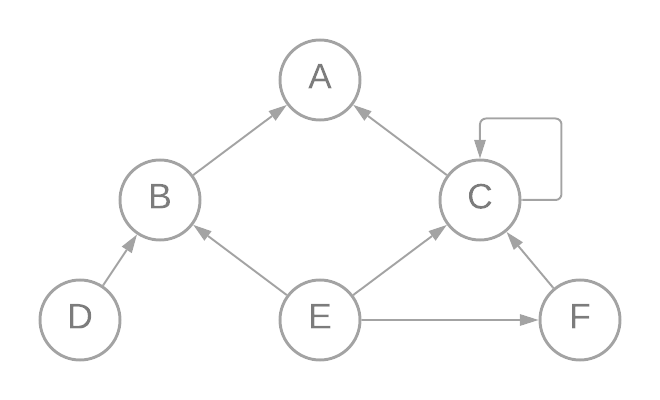
\includegraphics[width=\linewidth]{./truth-and-reconciliation-graph.png}
      \caption{Exchange of service graph}
      \label{figure:2}
    \end{figure}

    This graph shows how projects can build upon one another to deliver value to the business.
    For example, product E uses services provided by product B, C, and F.
    At the end of the day, we want to ensure product E is attributed the resources that they use.

\section*{Implementation}
  When it comes to implementation, I've found there are two schools fo thought.

  The first approach is to use real world dollars.
  This encounters many challenges such as choosing a base currency or determining the cost of non-cloud environments.
  In many ways, this information is extremely valuable for product owners.
  They understand what their system costs and how much they should expect to charge for their service.
  In the wrong hands, this information is dangerous.

  The second approach is to use a basis point type of system.
  This approach allows you to represent the underlying usage as a percentage.
  One problem with this approach is that when you scale a cluster up, usage goes down.
  If product owners look at raw basis points, they'll see a decrease in their usage.
  This can be really confusing if you haven't deployed changes recently.

  At the end of the day, we need a combination of these approaches.
  Basis points should be used to apportion out usage at each tier.
  When displaying or analyzing information, a currency value should be used.
  This approach allows for the most accurate representation of a given products cost.

  \subsection*{The Ledger}

    \begin{table}[H]
      \centering
      \begin{tabular}{ l|l }
        Field & Explanation \\
        \hline
        datetime & Time of transaction \\
        region & A geographic identifier \\
        env & An environmental identifier \\
        payer & Who received services (from) \\
        payee & Who provides services (to) \\
        type & A debit or credit \\
        amount & Amount of money (millicents) \\
        urn & A uniform resource name \\
        tags & Organization specific metadata \\
        detail & A break down of charges
      \end{tabular}
      \caption{Fields on each document}
      \label{table:1}
    \end{table}


  \subsection*{Apportioning Resources}

    Testing

  \subsection*{Over-commit}

    Over-commit puts infrastructure owners in a rather perca


\section*{Verification}

  As we are discussing a financial system, we have to discuss the math behind some of this.

  \[ resource = \{ measure, cost \} \]

  \[ costmodel = \{ resource, ... \} \]



\end{document}
